\documentclass[tikz]{standalone}
\usepackage{pgfplots}
\pgfplotsset{compat=1.15}
\usepackage{mathrsfs}
\usetikzlibrary{arrows,calc}
\usepackage{tkz-euclide}
\pagestyle{empty}

\definecolor{AngleClr}{rgb}{0,0.39215686274509803,0}
\definecolor{ShapeClr}{rgb}{0.6,0.2,0}
\definecolor{BlueClr}{RGB}{5,81,163}
\definecolor{RedClr}{RGB}{199, 28, 16}
\definecolor{YellowClr}{RGB}{191, 159, 0}

\begin{document}

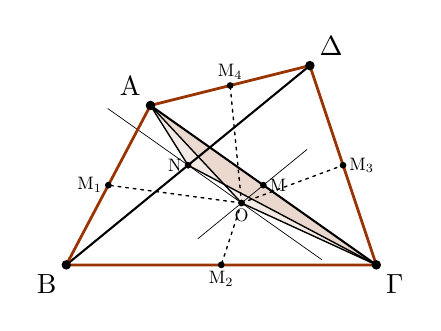
\begin{tikzpicture}[scale=.75]
\tkzSetUpLine[line width=1pt,color=black]
\tkzSetUpPoint[fill=black]

% \tkzDefPoints{0/0/B,3.5/0/C,0.95/1.8/A,2.75/2.25/D}
\tkzDefPoints{0/0/B,5.25/0/C,1.425/2.7/A,4.125/3.375/D}

\tkzDefMidPoint(A,B) \tkzGetPoint{M1}
\tkzDefMidPoint(B,C) \tkzGetPoint{M2}
\tkzDefMidPoint(C,D) \tkzGetPoint{M3}
\tkzDefMidPoint(D,A) \tkzGetPoint{M4}

\tkzDefMidPoint(A,C) \tkzGetPoint{M}
\tkzDefMidPoint(B,D) \tkzGetPoint{N}

\tkzDefLine[parallel=through N](A,C) \tkzGetPoint{NN}
\tkzDefLine[parallel=through M](B,D) \tkzGetPoint{MM}

\tkzInterLL(N,NN)(M,MM) \tkzGetPoint{O}


\tkzFillPolygon[fill=white](A,B,C,D,O)
\tkzFillPolygon[fill=ShapeClr,fill opacity=0.1](A,N,C)
\tkzFillPolygon[fill=ShapeClr,fill opacity=0.1](A,O,C)

\tkzDrawSegments[line width=0.25pt,add=1.5 and 1.5](N,O)
\tkzDrawSegments[line width=0.25pt,add=2 and 2](M,O)

\tkzDrawSegments[line width=0.75pt](A,C B,D)
\tkzDrawSegments[line width=0.5pt](A,N C,N A,O C,O)
\tkzDrawSegments[line width=0.5pt,color=black,dashed,dash pattern=on 1pt off 1.75pt](O,M1 O,M2 O,M3 O,M4)

\tkzDrawPolygon[color=ShapeClr](A,B,C,D)
\tkzDrawPoints[size=3](A,B,C,D)
\tkzDrawPoints[size=2](O,M1,M2,M3,M4,N,M)
\tkzLabelPoint[above left](A){$\mathrm{A}$}
\tkzLabelPoint[below left](B){$\rm B$}
\tkzLabelPoint[below right](C){$\rm \Gamma$}
\tkzLabelPoint[above right](D){$\rm \Delta$}

\tkzLabelPoint[below,scale=0.65](O){$\rm O$}
\tkzLabelPoint[right,scale=0.65](M){$\rm M$}
\tkzLabelPoint[left,scale=0.65](N){$\rm N$}

\tkzLabelPoint[left,scale=0.65](M1){$\rm M_1$}
\tkzLabelPoint[below,scale=0.65](M2){$\rm M_2$}
\tkzLabelPoint[right,scale=0.65](M3){$\rm M_3$}
\tkzLabelPoint[above,scale=0.65](M4){$\rm M_4$}

\end{tikzpicture}

\end{document}
